%!TEX root = ../TTK4550-MHT.tex
\section{Algorithm walk-through}
\label{sec:algorithm}
\subsection{Flowchart}
Figure \ref{fig:algorithm_flow} shows a flowchart of the \gls{tomht} algorithm presented in this section. An important difference between this approach compared to Reid's original \gls{homht} \cite{Reid1979}, is the need for external initialization of targets as mentioned in section \ref{subsec:tomht}.

\begin{figure}[H]
\centering
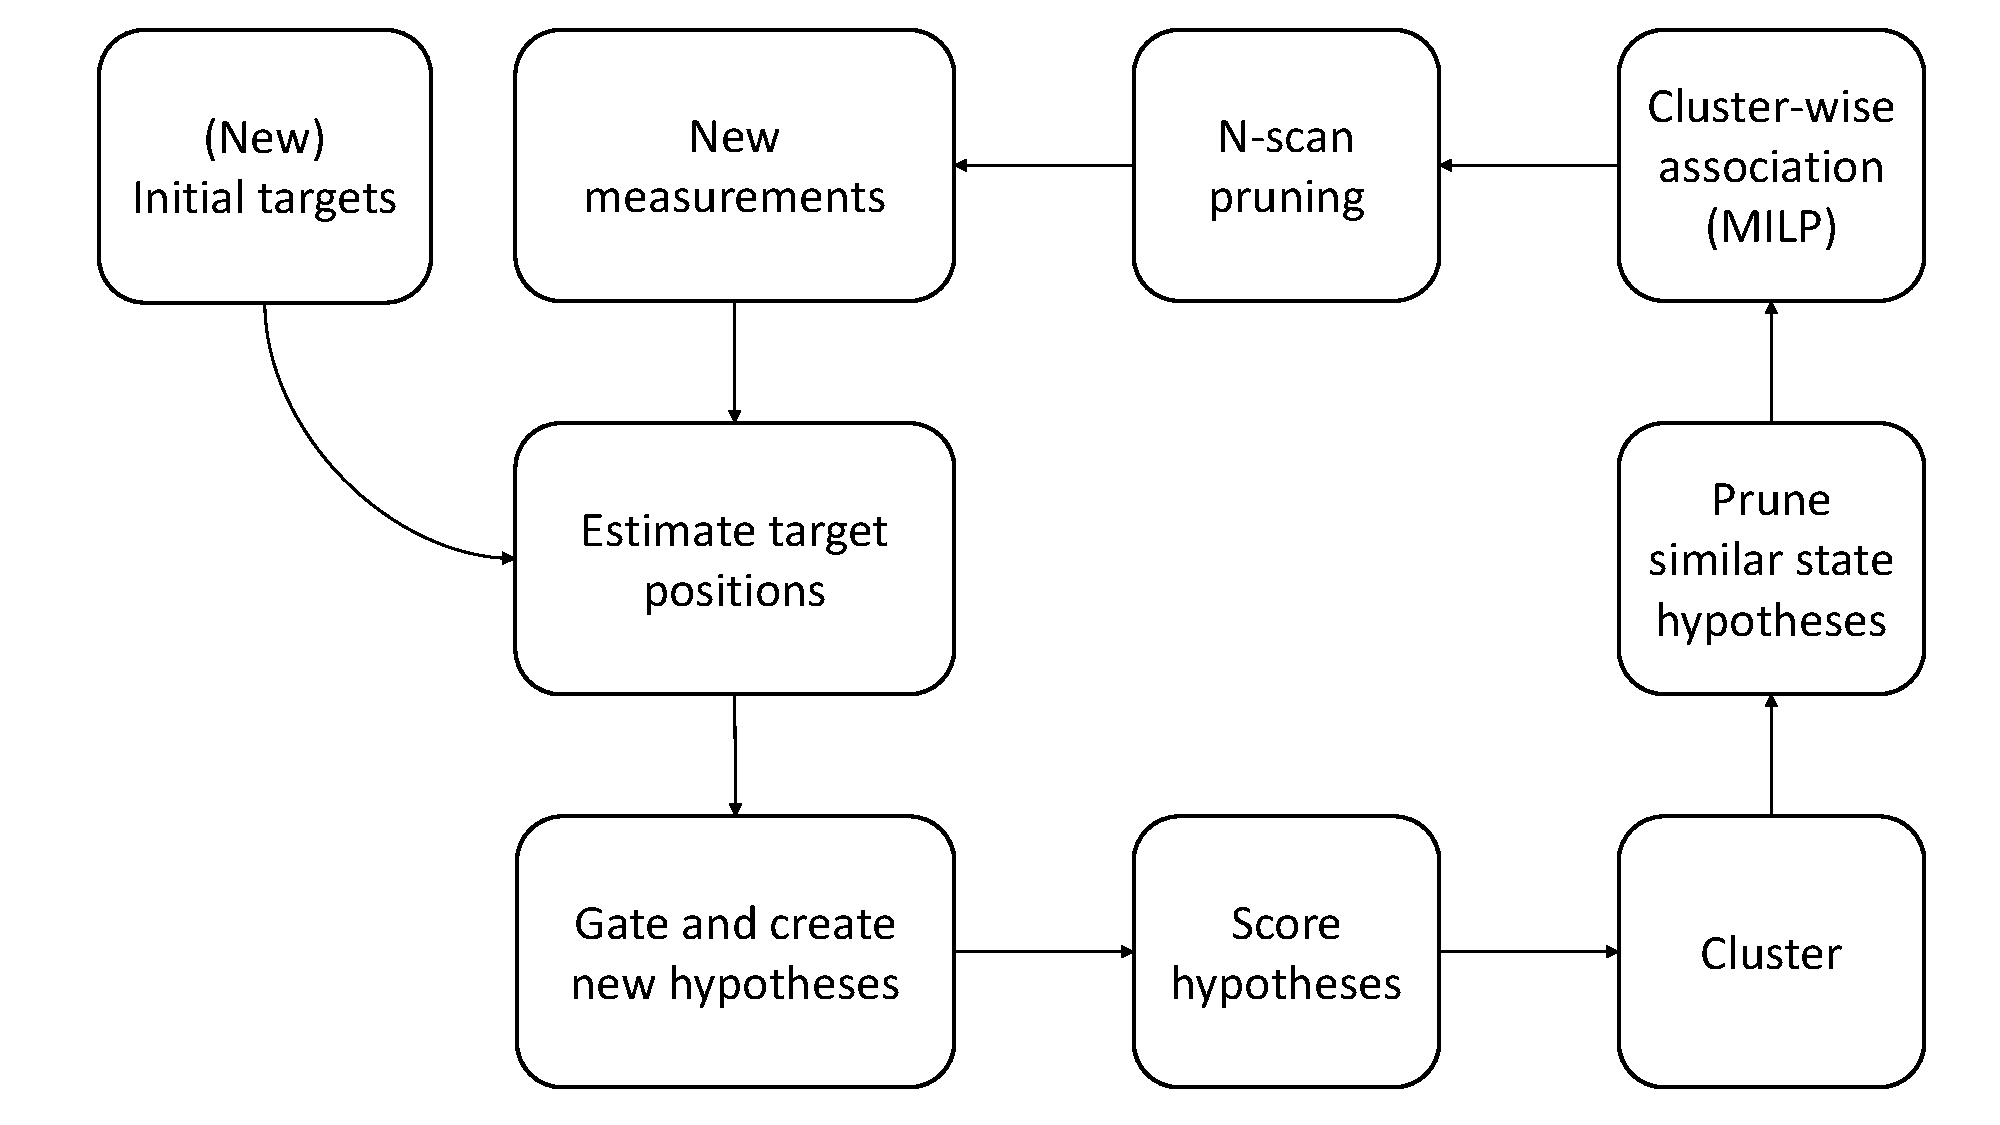
\includegraphics[width = .8\textwidth]{algorithm_flowchart.pdf}
\caption{Algorithm flowchart}
\label{fig:algorithm_flow}
\end{figure}

\subsection{State estimation} %TODO: Split up in modelling and estimation section
When a new set of measurement arrives, it is desirable to "guess" where the target might be before looking for matching measurements. This can be done though a model of the targets dynamics and a state estimator. For the purpose of tracking ships in a local frame (Cartesian plane), we compose a state vector with four states
\begin{equation}
\V{x} = \begin{bmatrix}
x & y & \dot{x} & \dot{y}
\end{bmatrix}^T
\label{eq:state_vector}
\end{equation}
where the change of velocity (acceleration) is assumed zero. The latest assumption is compensated with an increased system noise covariance in the model. For a linear system with white and uncorrelated system and measurement noise, the Kalman Filter is an optimal estimator with (\ref{eq:kalman_model}) as time evolution model,
\begin{equation}
\begin{split}
\V{x}(k+1) &= \M{\Phi} \V{x}(k) + \M{\Gamma} \V{w} \\
\V{z}(k) &= \M{H} \V{x}(k) + \V{v}
\end{split}
\label{eq:kalman_model}
\end{equation}
where
\begin{equation}
\begin{split}
\M{\Phi} 	&= \text{the state transition matrix} \\
\M{\Gamma}	&= \text{the disturbance matrix} \\
\V{w}		&= \text{the process noise} \\
\M{H} 		&= \text{the measurement matrix} \\
\V{v} 		&= \text{the observation noise} \\
\end{split}
\end{equation}.
The procedure of predicting the target state at the next time step is according to the "time update" equations of the Kalman Filter (\ref{eq:kalman_timeUpdate}),
\begin{equation}
\begin{split}
\V{\bar{x}}(k+1) 	&= \M{\Phi} \V{\hat{x}}(k) \\
\M{\bar{P}}(k+1)	&= \M{\Phi} \M{\hat{P}}(k)  \M{\Phi}^T + \M{Q} \\
\end{split}
\label{eq:kalman_timeUpdate}
\end{equation}
where $\M{Q}$ is the process noise covariance matrix. The model have the following parameters,
\begin{equation*}
\M{\Phi} =	\begin{bmatrix}
1 & 0 & T & 0 \\
0 & 1 & 0 & T \\
0 & 0 & 1 & 0 \\
0 & 0 & 0 & 1 \\
\end{bmatrix} \quad
\M{\Gamma} = \begin{bmatrix}
0 & 0 \\
0 & 0 \\
1 & 0 \\
0 & 1 \\
\end{bmatrix} \quad
\M{H} = \begin{bmatrix}
1 & 0 & 0 & 0 \\
0 & 1 & 0 & 0 \\
\end{bmatrix}
\end{equation*}
\begin{equation*}
\M{Q}	= \sigma_v^2 \begin{bmatrix}
\frac{T^3}{3} 	& 0 				& \frac{T^2}{2}	& 0 			\\
0 				& \frac{T^3}{3}  	& 0 			& \frac{T^2}{2}	\\
\frac{T^2}{2}	& 0					& T				& 0				\\
0				& \frac{T^2}{2}		& 0				& T				\\
\end{bmatrix} \quad
\M{R} = \sigma_r^2 \begin{bmatrix}
1 & 0 \\
0 & 1 \\
\end{bmatrix}
\end{equation*}
where $T$ is the time between the current and the previous measurement, $\sigma_v^2$ is the system velocity variance and $\sigma_r^2$ is the measurement variance. This model, known as the constant velocity model,  is very common due to its simplicity, and is used in among others \cite{Reid1979}, \cite{Coraluppi2000} and \cite{Brekke2012}.

\subsection{Gating}
To avoid calculating the likelihood for all possible combinations of targets and measurements, some sort of selection criteria is needed when creating new hypotheses. One way of doing this selections is to select all measurements that are within a certain confidence region or gate (\ref{eq:gate}), illustrated in Figure \ref{fig:validation_region}.
\begin{figure}[H]
\centering
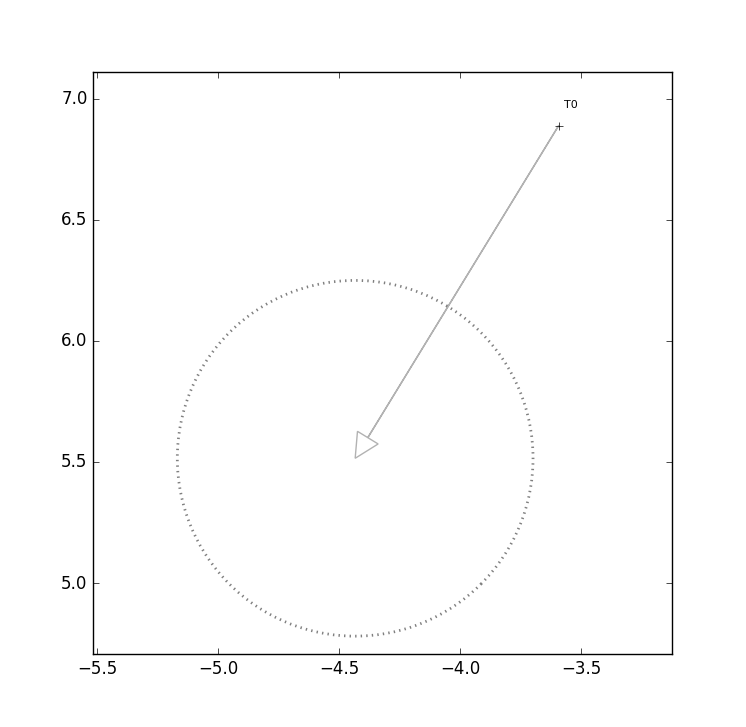
\includegraphics[clip, trim = 1.5cm 1cm 1.5cm 1.5cm,width = .6\textwidth]{ex1-validationRegion}
\caption{Validation region}
\label{fig:validation_region}
\end{figure}
\begin{equation}
\begin{gathered}
\M{B}	= \M{H} \M{\bar{P}} \M{H}^T + \M{R} \\
(\V{Z_m} - \M{H}\V{\bar{x}})^T	\M{B}^{-1} (\V{Z_m} - \M{H}\V{\bar{x}}) \leq \eta^2
\label{eq:gate}
\end{gathered}
\end{equation}

This is a very common approach, and is used by most tracking systems at some stage in the processing of new measurements. In (\ref{eq:gate}), $\eta$ is the inverse \gls{cdf} of the chi-square distribution for a given confidence with degrees of freedom equal to the sensor system. For each measurement inside the region, a filtered state and covariance is calculated using the "measurement update" equations in the Kalman Filter (\ref{eq:kalman_measurementUpdate}), followed by the creation of a new track hypothesis.
\begin{equation}
\begin{split}
\V{\tilde{y}}	&= \V{z} - \M{H} \V{\bar{x}} \\
\M{S}			&= \M{H} \M{\bar{P}} \M{H}^T + \M{R} \\
\M{K} 			&= \M{\bar{P}} \M{H}^T \M{S}^{-1} \\
\V{\hat{x}}(k) 	&= \V{\bar{x}} + \M{K} \V{\tilde{y}} \\
\M{\hat{P}}(k) 	&= \left( \M{I} - \M{K} \M{H} \right) \M{\bar{P}}
\end{split}
\label{eq:kalman_measurementUpdate}
\end{equation}

The $\chi^2$ value for selected confidence values are listed in Table \ref{tab:chi_square}, where $95\% - 99\%$ is a common interval for gate size. 
\begin{table}[H]
\centering
\begin{tabular}{c c c c c c c c}
Confidence 	& 70\% 	& 80\% 	& 90\% 	& 95\% 	& 97.5\% 	& 99\% 	& 99.5\% \\ \hline
$\eta^2$ 	& 2.41 	& 3.22 	& 4.61 	& 5.99 	& 7.38 		& 9.21 	& 10.60
\end{tabular}
\caption{Inverse $\chi^2$ \gls{cdf} for two degrees of freedom}
\label{tab:chi_square}
\end{table}

\subsection{Scoring}
Each track hypothesis are scored according to \cite{Bar-Shalom2007}:
\begin{equation}
\begin{split}
\mathrm{NLLR}_{i,j}(k) &= \frac{1}{2} \left[ {\tilde{y}_k^j}(i)^T {S_k^j}^{-1} {\tilde{y}_k^j}(i) \right] + \ln \frac{\lambda_{ex} |2 \pi S_k^j|^{1/2}}{P_D} \\				
\tilde{y}_k^j(i) &= z_k^i -\hat{z}_{k|k-1}^j
\end{split}
\end{equation}
The cumulative NLLR is then
\begin{equation}
\mathrm{cNLLR}_k^j \triangleq \sum_{l=0}^k NLLR_{i,j}(l)
\end{equation}

\subsection{Clustering}
Since the global problem of finding the optimal selection of hypotheses is growing exponentially with the number of hypotheses, it is computationally beneficial to split the problem into smaller problem. This can only be done to targets that does not share any measurements. The clustering can be done efficiently through breath-first-search or depth-first-search on a graph made from the hypothesis tree.

By constructing a 0-1 adjacency matrix describing the connection between all the nodes in the track forest, the clustering problem is equivalent to the \emph{connected components} problem in graph theory \cite{Chen2015}.

\subsection{Association}
When the targets are divided into independent clusters, each of them can be treated as a global problem where we want to minimize the cost or maximize the score of the selected track hypotheses (leaf nodes), while fulfilling the constraints that each measurement can only be a part of one track and that minimum and maximum one hypothesis can be selected from each target. Since only binary values, selected of not selected, is desired for selection of hypotheses, the problem becomes an \gls{ilp}. A solution to this problem is explained in section \ref{sec:ilp}.

\subsection{N-scan pruning}
To keep the computational cost within reasonable limits, it is necessary to limit the amount of time steps backwards in time that the algorithm computes. This is done by removing all branches but the active track hypothesis at the current root node, and assign the (one) remaining node as new root node. This procedure is graphically explained in Figure \ref{fig:pruned-hyp-tree}, where a solid square frame indicates the current root node, and a dotted square frame indicates the new root node. The bold arrows in the figure represents the active track.

A similar, and in scenarios with low \gls{Pd} perhaps better strategy, is N-\gls{observation} pruning proposed by \cite{Blackman2004}. The idea is to prune N \emph{measurements} back in time instead of N \emph{scans}. This approach will lead to larger and more costly track trees for tracks that have low probability of detection. Therefore, in any practical implementation a N-observation pruning scheme will be followed by a traditional M-scan pruning, where M is larger than N. The combination of these two methods can be seen on as a form of adaptive pruning where tracks with high probability of detection can manage with fewer history steps than tracks with low probability of detection.

\begin{figure}[ht]
\centering
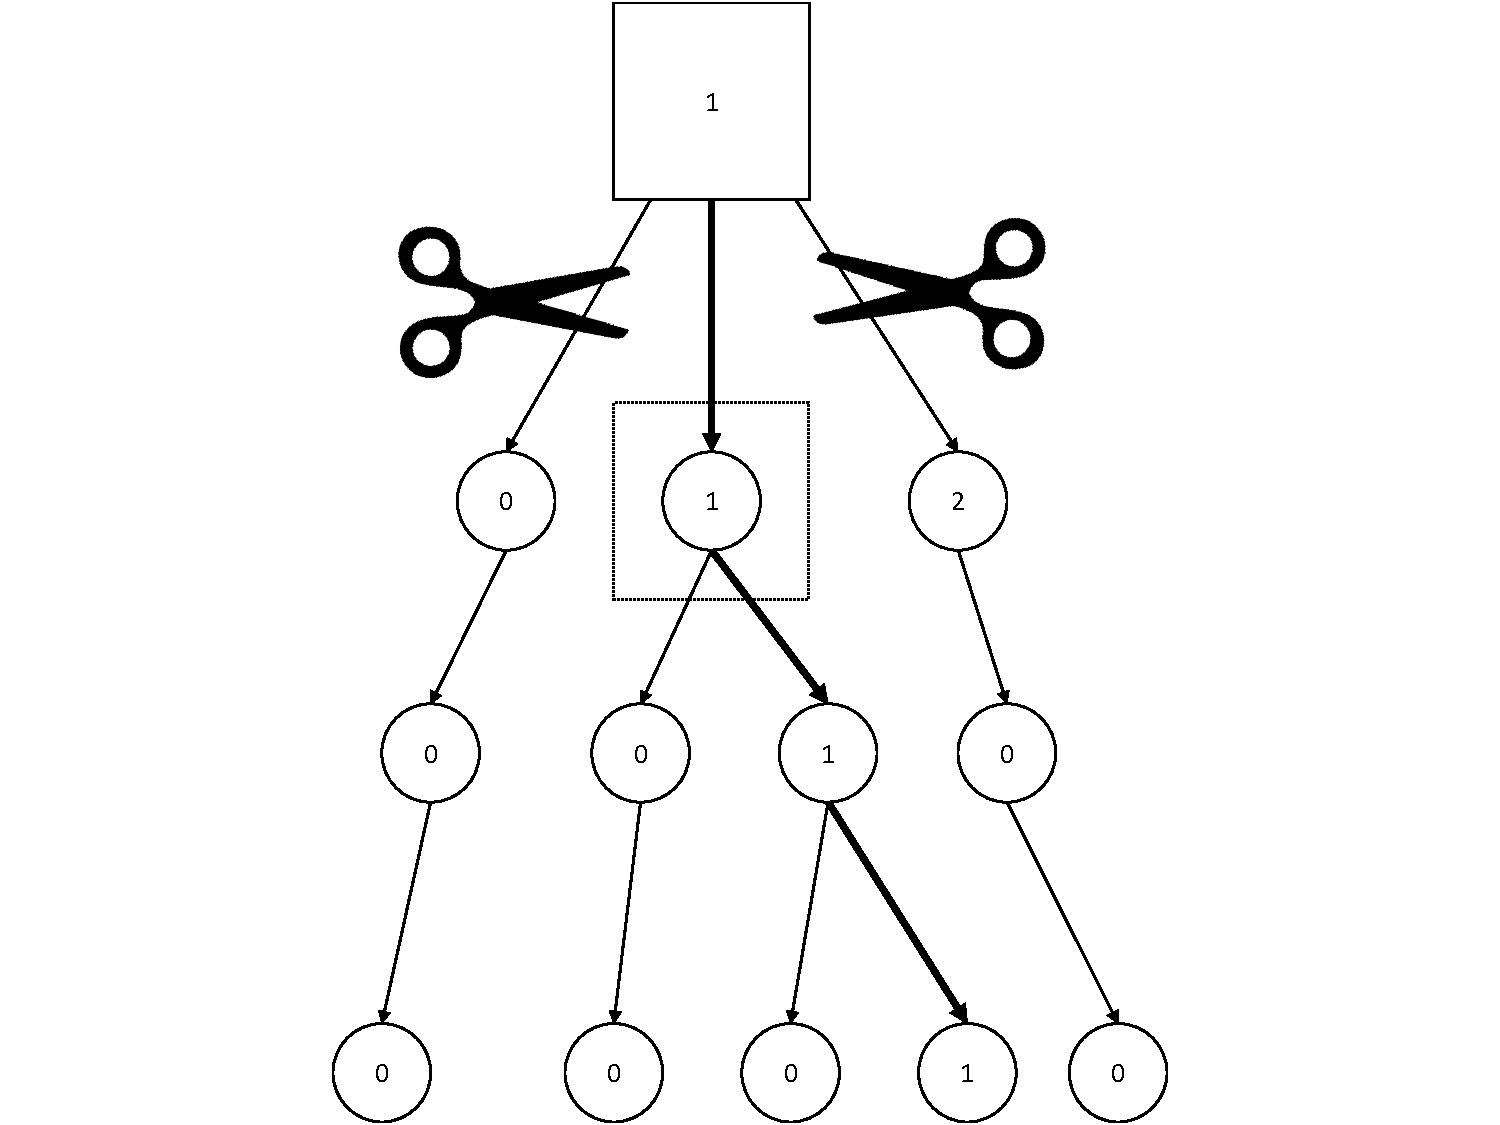
\includegraphics[clip, trim = 2cm 0cm 2cm 0cm,width = .7\textwidth]{Pruned-tree.pdf}
\caption{Pruned track hypothesis tree}
\label{fig:pruned-hyp-tree}
\end{figure}